\documentclass{article}
\usepackage[margin=1in]{geometry}
\usepackage{amsmath}
\usepackage{amssymb}
\usepackage{amsthm}
\usepackage{url}
\usepackage{todonotes}
\usepackage{svg}
\usepackage{cleveref}

% Environments

\newtheorem{theorem}{Theorem}
\newtheorem{proposition}[theorem]{Proposition}
\newtheorem{corollary}[theorem]{Corollary}
\newtheorem{lemma}[theorem]{Lemma}
\newtheorem{definition}[theorem]{Definition}
\newtheorem{conjecture}[theorem]{Conjecture}
\newtheorem{remark}[theorem]{Remark}


\theoremstyle{definition}
\newtheorem{example}[theorem]{Example}

\numberwithin{theorem}{section}
\numberwithin{equation}{section}

\DeclareMathOperator{\Int}{int}
\DeclareMathOperator{\Star}{st}
\DeclareMathOperator{\Lk}{lk}
\DeclareMathOperator{\Homeo}{Homeo}
\newcommand{\atlas}{\mathcal{A}}
\newcommand{\cover}{\widetilde{X}}

%opening
\title{Low Dimensional Topology}
\author{Eric Luu}

\begin{document}

\section{Sheet 1}


\subsection{Question 3}

\subsubsection{a}
Using the 1 point compatification, we have that the solid torus is produced of $S^3 - U$. Embed $U$ in $S^3$ on the $z$-axis, which passes through $\infty$. Then we have that $S^3 - U$ is simply $\mathbb{R}^3$ without the $z$-axis, which is homeomorphic to the solid torus. 
\subsubsection{b}
From above, we have that $\pi_1(S^3 - U) = \mathbb{Z}$ as this is the fundamental group of the solid torus. It can also be seen by the only nontrivial loop (up to homotopy) being ones which wrap around the hole left behind by $U$. 
\subsubsection{c}
Label one of the loops $U$ and the other loop $L$. We have that on the left the homotopy equivalence class of $L$ in $S^1 - U$ is nontrivial but on the right the homotopy class of $L$ in $S^1 - U$ is trivial. Therefore, we have that the left and the right cannot be equivalent as homeomorphisms sends homotopy equivalence classes to each other in the natural way. 

\subsection{6}
We have that $M(n)$ is a smooth manifold. Now consider the function $\det : M(n) \rightarrow \mathbb{R}$, which is a smooth function between two manifolds as it is a polynomial. Now look at $\det^{-1} (1)$, which is precisely the matrices of determinant $1$. Now we want to show that the Jacobian on this set is not the zero vector, so that the preimage is a submanifold. 

Then as we have that $(D \det A)_{ij} = (-1)^{i + j} \det(A^*_{i, j})$ where $A^*_{i, j}$ is the cofactor matrix of $A$ deleting $i$ and $j$. Then this means that this is zero iff the determinant of the cofactor matrix is zero, but this is never the case as the determinant of $A$ itself is nonzero, meaning $A$ is invertible and so are all of its cofactors. Therefore, $D \det(A)$ is 0 iff $\det A = 0$, meaning that the preimage is a submanifold. 

Finally, we have that the dimension is $n^2-1$ and the codimension is 1. 

\section{Sheet 2}

\subsection{2}
Show that $A \cup B$ is homeomorphic to $S^1$. Then use Schoenflies to show that $A \cup B$ has an interior and an exterior. Then use a homeomorphism taking $A \cup B$ to the disc, with one point at (1, 0) and another point at (-1, 0). The ambient isotopy should be easy to find at this point. 

\subsection{3}
Suppose Jordan Line Theorem is true. Let $L$ be a simple closed curve in $S^2$. Then take $N$ to be on $L$ and stereograph project to $L'$ in $\mathbb{R}^2$. Then $L'$ divides up plane to two halves by Jordan Line Theorem. Then we go backwards and project both the two components and $L$ back to $S^2$. 

Suppose Jordan Curve Theorem is true. Take line $L$ in $\mathbb{R}^2$. Then stereograph project $L$ to $S^2$. Will divide into two sections. Then stereograph project $L'$ and 2 components to $\mathbb{R}^2$.  

\subsection{4}
Consider thickening the plane in the $z$ axis by dragging it to $[-1,1]$ and letting the two open sets be $z > -1/2$ and $z < 1/2$ with intersection homeomorphic to the plane. 
\subsection{5}
Take any arc $L$ in $\mathbb{R}^3$ and a plane $P$. There is an isotopy of $P$ to the $xy$-plane. Then there exists an ambient isotopy from the arc to the $x$-axis. 

\subsection{6}

Take any arc and have an ambient isotopy from the plane to the $xy$-plane. Then there is an ambient isotopy to $S^1$. 


\section{3}

\subsection{1}
\subsubsection*{a}
Take a point $(e^{2\pi i \theta}, e^{2 \pi i \varphi})$ on $T^2 \cong S^1 \times S^1$ where $S^1 \subset \mathbb{C}$. The preimage of this set in $\mathbb{C}$ is $(m + \theta) + i (n + \varphi)$ where $m, n \in \mathbb{Z}$. Consider the open neighbourhood $U = (e^{2 \pi i (\theta - 1/100)}, e^{2 \pi i (\theta + 1/100)}) \times (e^{2 \pi i (\varphi - 1/100)}, e^{2 \pi i (\varphi + 1/100)})$. Then $p^{-1}(U)$ are the points $x + i y$ where $x \in (\theta + m -1/100, \theta + m + 1/100)$, $y \in (\varphi + n - 1/100, \varphi + n + 1/1000)$, and $m, n \in \mathbb{Z}$. Then the open sheets are of the form $U_{m,n} = \{x + i y : m + \theta - 1/100 \leq x \leq m + \theta + 1/100, n + \varphi - 1/100 \leq y \leq n + \varphi + 1/100\}$ for some $m, n \in \mathbb{Z}$. These sheets are disconnected for each $m, n$. Finally, $p|_{U_{m,n}}$ is the map from $(\theta + m -1/100, \theta + m + 1/100) \times (\varphi + n - 1/100, \varphi + n + 1/100)$ to $(e^{2 \pi i (\theta - 1/100)}, e^{2 \pi i (\theta + 1/100)}) \times (e^{2 \pi i (\varphi - 1/100)}, e^{2 \pi i (\varphi + 1/100)})$. This is a bijection and a homeomorphism, as $n \mapsto e^{2 i \pi n}$ is a homeomorphism on the range $[\theta - 1/100, \theta + 1/100]$ for any $\theta$. 

\subsubsection*{b}
$\exp$ is a continuous map as it is entire. Let $R e^{i \theta}$ be a point in $\mathbb{C} - 0$. The preimage of this point are the points $(\ln(R), \theta + 2 \pi z)$ where $z \in Z$.

\subsection{2}

\begin{theorem}
    Let $X$ be a topological space and let $p : \cover \rightarrow X$ be a covering space. Let $F: I \times I \rightarrow X$ be a homotopy of paths where $F(\cdot, 0) = \gamma_0$ and $F(\cdot, 1) = \gamma_1$ rel endpoints. Suppose $F(0,t) = x_0$ and $F(1, t)= x_1$. $\tilde{x}_0 \in p^{-1}(x_0)$ there exists a unique lifted homotopy $f_t: I \rightarrow \cover$ of paths starting at $x_0$.
\end{theorem}

\begin{proof}
    For each $F(s, t) \in X$, there exists open sheets $U_{F(s, t)}$ that contains $F(s, t)$ and is evenly covered. Because $F(s, t)$ is continuous, then $F^{-1}(U_{F(s, t)})$ are open in $I \times I$. By the compactness of $I \times I$, there exists a finite number of intervals $0 = s_0 < s_1 < \cdots < s_m = 1$ and $0 = t_0 < t_1 \ldots < t_n = 1$ such that intervals $[s_i, s_{i + 1}] \times [t_j, t_{j + 1}]$ is contained inside some $U_{F(s,t)}$.

    From the path lifting theorem, there exists a unique path $\widetilde{\gamma_0} : I \rightarrow \tilde{X}$ where $\widetilde{\gamma_0}(0) = \tilde{x}_0$. Now induct over $t_i$. Let $\gamma_i = F(\cdot, t_i)$. Suppose for induction, $\widetilde{\gamma_i}$ is the unique path of $\gamma_i$. Let $\widetilde{\gamma_i}(0) = \tilde{x}_0$. Then there exists a homotopy from $\widetilde{\gamma_i}$ to $\widetilde{\gamma_{i + 1}}$. Consider $[0, s_1] \times [t_i, t_{i + 1}]$. Then there exists a neighbourhood $U_{s, t}$ which contains $ \tilde{x}_0$ where $[0, s_1] \times [t_i, t_{i + 1}]$. Now define the path \todo{finish later!}
\end{proof}

\section{4}
\subsection{2}
Let $K$ and $K'$ be two null-homotopic knots on $T^2$. Then there exists an ambient isotopy of $T^2$ taking $K$ to $K'$.

Let $h : \mathbb{C} \rightarrow T^2$ be the standard covering map.  Without loss of generalisation, suppose $K'$ lifts to a simple closed curve in $\{x + i y : x \in [0, 1], y \in [0, 1]\} \subset \mathbb{C}$. 
Since $K$ and $K'$ are null-homotopic, they lift to loops $\widetilde{K}, \widetilde{K'}$  in $\mathbb{C}$ from Hatcher 1.31. There exists an ambient isotopy from $\widetilde{K}$ to $\widetilde{K'}$ by 2.10. Furthermore, there is a homeomorphism from $\widetilde{K'}$ to $K'$ as it lies in a fundamental region.  

Then there exists an ambient isotopy $\gamma$ in $\mathbb{C} \cong \mathbb{R}^2$ from $\widetilde{K}$ to $\widetilde{K'}$ by Corr 2.6. Therefore, $h \circ \gamma \circ h^{-1}$ is an ambient isotopy from $K$ to $K'$. This map is well-defined as $h|_{\gamma \circ h^{-1}(K')}$ is a homeomorphism. By the equivalency of ambient isotopy, any two null-homotopic knots are ambient isotopic. 

Note that $T^2$ can be replaced by any surface $S$ which have a universal cover of $\mathbb{C}$ or $\mathbb{R}$. 

\subsection{3}
Show that the homeomorphisms isotopic to the identity is a normal subgroup and that two maps are isotopic iff they are in the same coset mod identity homeomorphisms.
Firstly, we will show that $N$ is a subgroup of $\Homeo(S)$. Firstly, if $g \in N$, then $g^{-1} \in N$. Let $H(x, t) : S \times I \rightarrow S$ be an isotopy where $h_0 = Id$ and $h_1 = g$. Then $G(x, t) = h_1^{-1}(H(x, 1-t))$ is a continuous map by composition. Furthermore, $G(x, 0) = h_1^{-1}(H(x, 1)) = Id$ and $G(x, 1) = h_1^{-1}(H(x, 0)) = g^{-1}$. Therefore, $g^{-1}$ is isotopic to $N$. If $f$ and $g$ are isotopic to $N$ with isotopies $F$ and $G$ with $F_1 = f$, $G_1 = g$, $F_0 = G_0 = Id$, then $f \circ g$ is isotopic to $Id$ with isotopy:
\begin{equation*}
    H(x, t) =
    \begin{cases}
        F(x, 2t) & 0 \leq t \leq 1/2\\
        G(F(x, 1), 2t-1) & 1/2 \leq t \leq 1
    \end{cases}
\end{equation*}
This is continuous as this is a composition of continuous functions and at time $t = 1/2$, the two maps agree. At time $t = 0$, $H_0 = Id$ and at $t = 1$, $H_t = g \circ f$. Therefore, if $f, g \in N$, then $g \circ f \in N$. 

Now we will show that $N$ is normal in $\Homeo(S)$. 
Let $f \in \Homeo(S)$, $g \in N$. Then $f g f^{-1} \in N$. Let $G: S \times I \rightarrow S$ be an isotopy with $G_0 = Id$, $G_1 = g$. Then $H(x, t) = f \circ G(\cdot, t) \circ f^{-1} (x) $ is an isotopy. Firstly, $H(x, t)$ is continuous as it is a composition of continuous functions for fixed $x$ and fixed $t$. Then $H(x, 0) = f \circ g_0 \circ f^{-1} = f \circ Id \circ f^{-1} = f \circ f^{-1} = Id$. Then $H(x, 1) = f \circ g_1 \circ f^{-1} = f \circ g \circ f^{-1}$. Therefore, $f \circ g \circ f^{-1} \in N$. Therefore, $N$ is normal.

Finally, suppose $f$ is isotopic to $g$. Then $f^{-1} g \in N$. Take an isotopy $F : S \times I \rightarrow S$ where $F_0 = f$ and $F_1 = g$. Then take $H(x, t) = f^{-1}(F(x, t))$. This is continuous, as this is the composition of two continuous functions. Then $H_0 = f^{-1} \circ f = Id$ and $H_1 = f^{-1} \circ g$. Therefore, $f$ and $g$ are in the same coset. 

Suppose $f^{-1} g \in N$. Then there exists a isotopy $F : S \times I \rightarrow I$ where $F_0 = Id$ and $F_1 = f^{-1} g$. Then take $H = f \circ F$. This is continuous as it is the composition of two continuous functions. Furthermore, $F_0 = f \circ Id = f$ and $F_1 = f \circ f^{-1} \circ g = g$. Therefore, $f$ and $g$ are isotopic.  

\subsection{4}
We want to show that $GL(2, \mathbb{Z})$ is generated by $
\begin{bmatrix}
    1 & 1\\
    0 & 1\\
\end{bmatrix},
\begin{bmatrix}
    1 & 0\\
    1 & 1\\
\end{bmatrix},
\begin{bmatrix}
    0 & 1\\
    1 & 0\\
\end{bmatrix}$. We want to show that any matrix in $GL(2, \mathbb{Z})$ can be reduced to the identity by applying a series of the matrices above, and then taking the inverse of the operations to build back the matrix. 
Suppose $\begin{bmatrix}
    a & b\\
    c & d\\
\end{bmatrix} \in GL(2, \mathbb{Z})$. Therefore, $ad - bc = \pm 1$.

If $A = \begin{bmatrix}
    a & b\\
    c & d\\
\end{bmatrix}$
has determinant $-1$, then 
$\begin{bmatrix}
    a & b\\
    c & d\\
\end{bmatrix} 
\begin{bmatrix}
    0 & 1\\
    1 & 0\\
\end{bmatrix}
=
\begin{bmatrix}
    b & a\\
    d & c\\
\end{bmatrix}
$ has determinant 1. Therefore, consider the case when $ad - bc = 1$.

If $|a| > |c| > 0$, then do the operation:

\begin{equation*}
    \begin{bmatrix}
        1 & \pm 1\\
        0 & 1
    \end{bmatrix}
    \begin{bmatrix}
        a & b\\
        c & d\\
    \end{bmatrix}
    = 
    \begin{bmatrix}
        a \pm c &b\\
        c & d
    \end{bmatrix}
\end{equation*}
so that $|a \pm c| < |a|$.
If $|a| \leq |c| > 0$, then do the operation:
\begin{equation*}
    \begin{bmatrix}
        1 & 0\\
        \pm 1 & 1
    \end{bmatrix}
    \begin{bmatrix}
        a & b\\
        c & d\\
    \end{bmatrix}
    = 
    \begin{bmatrix}
        a &b\\
        c \pm a & d
    \end{bmatrix}
\end{equation*}
such that $|c \pm a| < |c|$. Repeat this operation until the matrix becomes:
\begin{equation*}
    \begin{bmatrix}
        \gcd(a, c) & x\\
        0 & y\\
    \end{bmatrix}
\end{equation*}
for some $x, y \in \mathbb{Z}$. However, $ad - bc = 1$. As $ax - yc = k \gcd(a, c)$ over $\mathbb{Z}$ for some $k \in \mathbb{Z}$, then $\gcd(a, c) = 1$. Therefore, 

\begin{equation*}
    A' = \begin{bmatrix}
        1 & x\\
        0 & y\\
    \end{bmatrix}
\end{equation*}
However, $\det(A') = 1$ as $A'$ is the composition of matrices with determinant 1. Therefore, $y = 1$. Therefore, $A'$ is of the form

\begin{equation*}
    \begin{bmatrix}
        1 & x\\
        0 & 1\\
    \end{bmatrix}
\end{equation*}
for some integer $x \in \mathbb{Z}$. But $
\left(\begin{bmatrix}
    1 & 1\\
    0 & 1\\
\end{bmatrix}\right)^x = \begin{bmatrix}
    1 & x\\
    0 & 1\\
\end{bmatrix}$. Therefore, $A$ can be composed from the above three matrices. 

\subsection{5}
Call all homeomorphisms isotopic to $id$ null-isotopies. 

Between any two points $p_0, p_1 \in S^2$, there is a null-isotopy such that $f(p_0) = p_1$. This is done by rotating the sphere around. 

Take any $f$ which is orientation preserving. Then pick a point $p_0$. Then there exists a null-isotopy $\gamma : S^2 \rightarrow S^2$ such that $\gamma(f(p_0)) = p_0$, through a rotation of the sphere. Then $ \gamma \circ f$ is an isotopy that takes $p_0$ to $p_0$ (This step could be simplified with a Brower-type proof). However, $S^2 \cong D^2/{\partial D^2}$. Consider the quotient map $q : D^2 \rightarrow S^2$, where $p_0$ is the point on $\partial D^2$. Let $g : D^2 \rightarrow D^2$ such that $g \circ q = \gamma \circ f$. This map exists as $\gamma \circ f$ keeps $p_0$ fixed and changes $S^2 - \{p_0\}$, so $g = \gamma \circ f$ on the open disk under the map. Then $g|_{\partial D^2} = Id$. Then by Alexander's isotopy lemma, $g$ is an isotopy. Therefore, $\gamma \circ f$ is also an isotopy, therefore $f$ is an isotopy. Thus shown. 

Orientation-reversing homeomorphims cannot be transformed to orienting preserving homeomorphisms on $S^2$. 


\newcommand*{\inter}{\hat{i}}
\newcommand*{\twequiv}{\sim_c}
\section{5}


\subsection{4}
\subsubsection{a}

Let $T_a$, $T_b$ be two Dehn twists around simple closed curves.

If $a$ and $b$ are essential and do not intersect, consider $S - a \cup b$ be a cut along $a$ and $b$. Then this cut has halves $b_1$ and $b_2$ which are glued together to form $S - a$. Then if $b_1$ and $b_2$ are on the same component of $S - a \cup b$, draw an arc $c$ from $b_1$ to $b_2$ at points which are identified to be the same point in $S$. Then as $c$ only touches $b$ once, $i(b, c) = 1$ as there is no operation to turn a single crossing into no crossing, and $i(a, c) = 0$. 

Now suppose if $b_1$ and $b_2$ are on different components $S_1, S_2$. Since $b$ is essential, $S_1$ and $S_2$ contain a either boundary components or a handle. Then there is an arc that can be drawn on $S_1$ to two points $s_1, s_2$ on $b_1$ that either goes through a handle or around a disk. Do this for $s_1$ and $s_2$ on $S_2$. Call this curve $c$.

If either $S_1$ or $S_2$ have a handle, then $c$ will go on the handle. Then $c$ and $b$ do not form a bigon and therefore must intersect at least once. Then if either $S_1$ or $S_2$ have more than 2 holes, then $c$ cannot be moved through $a$ to not intersect $b$, by going around both holes. Since $a$ is not equal to $b$, neither $S_1$ nor $S_2$ is a disk, so there must be either two holes in one component as the total number of holes on the surface is at least 3 if there are no handles. Therefore, $c$ does exist. 
\subsubsection{b}
Let $c$ be a curve which follows $a$ but does not cross $a$. Then $c$ will cross $b$ near where $a$ crosses $b$. Thus shown. 

\subsubsection{c}
Let $a$ and $b$ be curves. Take $c$ to be the curve from part a or b, so $i(a, c) = 0$ and $i(b, c) \neq 0$. Then $i(T_a(c), c) = i(a, c)^2 = 0$, but $i(T_b(c), c) = i(b, c)^2 \neq 0$. This is from part 3. 
\subsection{d}
Suppose $a = b$. Then $T_a = T_b$ up to isotopy. Now suppose $a \neq b$. Then there exists a curve $c$ such that $i(T_a(c), c) = 0$ but $i(T_b(c), c) \neq 0$. Therefore, $T_a \neq T_b$ as it does not preserve the intersection number of curves up to isotopy. Thus shown both directions.

\subsection{5}
\subsubsection{a}

Let $f \in MCG(S)$. Let $a, b$ be isotopy classes of $SCC$ in $S$. Show $T_{f(a)} f = f T_a$. Hit both sides with $b$. Then $T_{f(a)} f(b)$ is a Dehn twist of $f(b)$ around $f(a)$. $T_a b$ is a Dehn twist of $b$ around $a$. However, outside of a neighbourhood of $f(a)$, $T_f(a) f(b) = f(T_a(b))$. Therefore, what is important is what goes on inside the neighbourhood of $b$. By homeomorphisms, $f(a \cap b) = f(a) \cap f(b)$. Therefore, the places where the point twists right are the same in both sections. Therefore, $T_{f(a)} f = f T_a$ and $T_{f(a)} = f T_a f^{-1}$. 

\subsubsection{b}

If both $a$ and $b$ are nonseparating, there exists a homeomorphism $f$ from $S^2 \rightarrow S^2$ that takes $a$ to $b$, by sheet 5, question 6. Then $T_b = f T_a f^{-1}$. 

\subsubsection{c}

If $f$ commutes with $T_a$, then $T_{f(a)} = T_{a}$. Therefore, $f(a) = a$. If $f(a) = a$, then $T_{f(a)} = T_{a}$. Therefore, $T_{f(a)} = f T_{a} f^{-1} = T_a$, so $f T_a = T f_a$.

\subsection{6}

\subsubsection{Reflexive}
For all scc $a$, $a \twequiv a$, through no twists.

\subsection{Symmetric}
Suppose $a \twequiv b$ through $b = T_1 T_2 ... T_m a$. Then $a = T_m^{-1} ... T_1^{-1}b$. This comes out of $T_i$ being a group element in $MCG^+(S)$ so group elements are associative and have inverses. Additionally, the inverse of $T_i$ is $T_i^{-1}$, the left Dehn twist as applying both to any curve returns something isotopic to the original curve. 

\subsubsection{Transitive}
Let $a, b, c$ be curves such that $a \twequiv b$ and $b \twequiv c$. Then $a \twequiv c$. 

Let $a = T_1 T_2 ... T_m b$ and $b = T_{m + 1} T_{m + 2}... T_{m + n} c$. Then $a = T_1 T_2 ... T_m T_{m + 1} ... T_{m + n} c$. Therefore, $a \twequiv c$. This comes from $T_i$ being a 

\subsection{7}

\subsubsection{a}
If $p$ is disjoint from $H_i$ then $P$ lives on the component of $S - c_1, ..., c_g$ homeomorphic to the sphere with $g$ holes. As every scc on a sphere minus holes is separating, $p$ must be separating. 

\subsubsection{b}
\paragraph*{i}
Suppose $p \subseteq H_i$ for some $H_i$. Then use the diagrams!!!


\paragraph*{ii}

Use more diagrams!


\section{6}

\subsection{1}
Show that $M_1 \cup_f M_2$ is a 3-manifold and orientable. 

We will first show $M_1 \cup_f M_2$ is locally Euclidean. Any point in the interior of $M_1$ or $M_2$ is in an open neighbourhood homeomorphic to an open ball, by $M$ being a manifold. Every point on $\partial M_1$ has a neighbourhood $N$ homeomorphic to an open set in $H^3$, the $3$-half plane with the subset topology of $\mathbb{R}^3$. As $f$ is a homeomorphism on $\partial M_1 \rightarrow \partial M_2$, $f|_{\partial N}$ has a corresponding open and connected neighbourhood $K$ in $\partial M_2$. Take any neighbourhood $N'$ homeomorphic to an open neighbourhood in $H^3$ in $M_2$ where $K = N' \cap \partial M_2$ (which exists as $K$ is continuous). Then $N \cup_f N'$ is an open neighbourhood around $p$. Furthermore, as $N$ and $N'$ are homeomorphic to open subsets of $H^3$ with neighbourhoods homeomorphic on $\partial H^3$, then gluing these along the homeomorphisms is an open disk in $\mathbb{R}^3$. Therefore, $M_1 \cup_f M_2$ is locally Euclidean.

Secondly, $M_1 \cup_f M_2$ is Hausdorff. By the quotient map, the union of the interior of $M_1$ and $M_2$ is Hausdorff, and every point in $M_1$ with a point on the boundary of $M_1$ have disjoint neighbourhoods as $M_1$ is Hausdorff. Furthermore, any two points on $\partial M_1$ and $\partial M_2$ are Hausdorff, as we take the intersection of Hausdorff open sets in $M_1$ and $M_2$. We can do this as $\partial M_1$ and $\partial M_2$ are homeomorphic. Therefore, $M_1 \cup_f M_2$ is Hausdorff. 

The union of bases for $M_1 \sqcup M_2$ is a basis for $M_1 \cup_f M_2$. As this is second-countable, so is $M_1 \cup_f M_2$. Therefore, $M_1 \cup_f M_2$ is a $3$-manifold.

To show orientability, take an orientation of $M_1 \sqcup M_2$. Since we glue outward normals to inward normals, we glue counterclockwise faces to clockwise faces in the simplicial approximation of $M_1$ and $M_2$. Therefore, the orientation given by $M_1$ is compatible with the orientation of $M_2$, therefore $M_1 \cup_f M_2$ is orientable. 

\subsection{3}

\paragraph*{$2 \Rightarrow 1$} Suppose $\gamma$ bounds a disk $D^2 \subseteq V$. Now take the deformation retraction $f : D^2 \times I \rightarrow D^2$ by the function $f(x, t) = xt$. At time $t = 1$, this is the identity map, but at time $t = 0$, this sends the disk to a single point. This is also a homotopy of $\partial D^2$ to a point. Therefore, $\gamma = \partial D^2$ is homotopic to a point on $D^2$, therefore it is homotopic to a point on $V$.

\paragraph*{$3 \Rightarrow 2$} Take the image $h({1} \times D^2)$. The boundary of this image is $\gamma$ and as this is a framing then the image is homeomorphic to a disk. Therefore, $\gamma$ bounds a disk in $V$.

\paragraph{$2 \Rightarrow 3$} Cut $V$ along $\gamma$ and the disk it bounds. Then this is a 2-ball, where $\gamma$ is on the boundary of the $2$-ball twice. By the annulus theorem, there exists a homeomorphism of the closed cylinder $D^2 \times I$ that takes $\partial D^2 \times {0}$ to one copy of $\gamma$ and $\partial D^2 \times {1}$ to another copy of $\gamma$. Gluing these two disks togehter in $D^2 \times I$ in the orientable way yields a framing $h : S^1 \times D^2$ where $h(\{1\} \times \partial D^2) = \gamma$. 

\paragraph{$1 \Rightarrow 2$} Let $f : S^1 \rightarrow V$ be a null-homotopic map, so there exists an $F: S^1 \times I \rightarrow V$ be a homotopy from $f$ to $V$. Now $F(x, 1) = x_1$ for all $x \in S^1$. Futhermore, the space $S^1 \times I$ where $S^1 \times \{1\}$ is homeomorphic to $D^2$. Therefore, $F : D^2 \rightarrow V$ is a map where $\gamma = \partial D^2$ is the map, therefore $\gamma$ bounds a disk in $V$.

\subsection{4}
\paragraph{$1 \Rightarrow 2$} Suppose $\gamma : S^1 \rightarrow V$ is a 

\subsection{5}

There is an ambient isotopy $h : \partial V \times I \rightarrow \partial V$ such that $h(\alpha, 1) = \beta$, as all meridians on the torus are ambient isotopic. But this induces an isotopy from $h_0 = Id$ to $h_1$ which is a homeomorphism from $\alpha$ to $\beta$. Therefore, $h_t$ can be extended to be a homeomorphism from a disk in $\alpha$ to a disk in $h_t(\alpha)$. Using Alexander's isotopy lemma from the identity to $h_1$, $h : \partial V \cup D^2 \times I \rightarrow \partial V$ is an ambient isotopy. Then if we cut $V$ along $D$, then this is a closed ball $B$, so $h$ has an extension from the boundary of the ball to the whole ball by Alexander's isotopy. Now because $\alpha$ becomes two circles on $B$, then we use the annulus theorem to split $\partial B$ into two disks and an annulus. Since $h: \partial B_n \rightarrow \partial B_n$ takes both copies of $\alpha$ to both copies of $\beta$ in the cut, then it also takes disks to disks and therefore this is an ambient isotopy. Therefore, we can extend $h : B_n \times I \rightarrow B_n$ for an ambient isotopy of $B_n$ from $Id$ to a map which takes both copies of $\alpha$ to $\beta$. Gluing along the boundaries again, we get a map $V \times I \rightarrow V$ that takes $\alpha $ to $\beta$. 

\subsection{6}
\subsubsection{a}
One pair of relatively prime integers that gives a longitude of $V$ is $\langle 1, 1\rangle$. 
\subsubsection{b}
\begin{lemma}
    A curve $\langle a, b \rangle$ on the torus $T^2$ intersects a particular meridian exactly once if and only if $|a| = 1$. 
\end{lemma}

\begin{proof}
    Consider the universal cover, $\mathbb{R}^2 \rightarrow T^2$. The curve $\langle a, b \rangle$ lifts to a curve which starts at $(0,0)$ and goes to $(a, b)$. Now draw lines when $x = \frac{1}{2}$. This is the preimage of the meridian in $\mathbb{R}^2$. TTherefore, $\langle a, b \rangle$ intersects the meridian exactly once if and only if $|a| = 1$. Thus shown. 
\end{proof}

\begin{theorem}
    $\zeta$ is a longitude if and only if the intersection number with the class of meridians up to isotopy is 1. 
\end{theorem}

\begin{proof}
    Since meridians are ambient isotopic, then moving meridians around, $i(\zeta, [m]) = 1$ for all $m$. 
\end{proof}

Therefore, $\langle a, b \rangle$ is a longitude is a meridian if and only if $a = 1$, $b \in \mathbb{Z}$. 

\subsection{7}

Every longitude is of the form $h(S^1 \times 1)$ for some framing $h$, therefore every longitude is homeomorphic to $S^1 \times 1$. Therefore, all longitudes are homeomorphic. 

Now consider longitudes $\langle 1, a \rangle $ and $\langle 1, b \rangle$ where $a, b \in \mathbb{Z}$ and $a \neq b$. Then there is no isotopy from $\langle 1, a \rangle$ to $\langle 1, b \rangle$ on $\partial V$ by the classification of curves on the torus. 

If two curves are ambient isotopic on $V$, then there exists an isotopy $F: V \times I \rightarrow V$ where $F_0 = Id$ and $F_1(\gamma) = \zeta$. But we can project from $V$ to $\partial V$ by having the homotopy take place on all but a circle in $V$. Then this is an isotopy on $\partial V$. Therefore, no isotopies on $\partial V$ implies there is no ambient isotopy on $V$ for $\langle 1, a \rangle$ and $\langle 1, b \rangle$. Thus shown. 

\subsection{10}

Cut the sphere into sections with radius $\frac{2\pi}{p}$. Start at the point $(0, 1, 0)$ and label the sections going counterclockwise $1 ... p$. Then section $1$ on the top is glued to $q + 1$ on the bottom, in this construction. Now cut out the cylinder $x^2 + y^2 \leq \frac{1}{4}$. This cylinder is a torus $V_1$ but with a twist of $\frac{p}{q}$ around the centre.

The shape left by removing this cylinder from the sphere is also a torus $V_2$. $V_2$ can be viewed as rotating each section around and gluing together to form a big wheel. However, there is still a longitudinal loop that is noncontractible in this big wheel by traversing through every shape. Since this space was connected before the quotient map, it is still connected after. 

Now let the section $x^2 + y^2 = \frac{1}{4}, z^2 = 3/4$ be the meridian of $V_1$. Then this curve runs along the edge of $V_2$ as well. Now the number of twists that it does is $p$ longitudinal curves and $q$ meridinal curves, as the top and the bottom are twisted around by $q/p$ full turns. Therefore, the meridinal curve is a $p, q$ curve on $V_2$. Since by definition, $p$ and $q$ are coprime, then $p$ and $q$ are the only unique natural numbers that fulfil this definition. 

We assume that $p > 0$ always. If this is not the case, then the manifold is $S^2 \times S^1$. 

\section{7}

\subsection{1}
We strengthen the induction assumption. Suppose $X$ and $Y$ are surfaces of genus $g$ and there exists a $h: \partial X \rightarrow \partial Y$. Then there is a $f : X \rightarrow Y$ homeomorphism where $f|_{\partial X}= h$. 

Let $X, Y$ be two handlebodies of genus $0$. Then $X$ and $Y$ are $3$-balls and are therefore homeomorphic. Furthermore, any homeomorphism on the boundary of the $3$-ball has an extension to $X$. Suppose this holds for all surfaces $< g$. Now suppose $X$ and $Y$ are two handlebodies of genus $g$. There exists a homeomorphism $h: \partial X \rightarrow \partial Y$ from the classification of surfaces. Now take a meridian $m$ in $X$. Now $m$ bounds a disk $D$ in $X$, therefore there is an extension of $h$ to $\partial X \cup D \rightarrow \partial Y \cup h(D)$. Cut $X$ along $D$ and $Y$ along $h(D)$. Then these two surfaces are of genus $g-1$. Then there exists an extension of $h$ on this surface to the cut $X$ and cut $Y$. Call this homeomorphism $f : X \setminus D \rightarrow Y \setminus h(D)$. Then taking the quotient space of $D$ to itself, $f$ is a homeomorphism from $X$ to $Y$. Therefore, $X$ and $Y$ are homeomorphic. 


\subsection{6}

Let $h$ be a homeomorphism of $H_1$ taking the images of meridians to itself. First cut along $f(m_1), ..., f(m_g)$ in $\partial H_1$. Call this shape $X$. Now $h$ restricted to $(X, \partial X)$ is a homeomorphism. Now this means that cutting along $h(m_1), ..., h(m_g)$ in $\partial H_1$ yields $(X, \partial X)$. 
Now in $H_2$, cut along $m_1$. Call this shape $Y$. Then the shape $H_1 \cup_f H_2$ can be viewed as taking $X \cup_f Y$ and regluing along meridians in $Y$ and $X$. But $X \cup_f Y \cong X \cup_h Y$ as there is a homeomorphism of $Y$ preserving boundary. Therefore, $H_1 \cup_f H_2 \cong H_1 \cup_h H_2$. 


\section{8}

\subsection{1}

\subsection{2}
Recall that $S^3 - V$ where $V$ is a solid torus is also a solid torus. Call $V_1 = N(K)$ and $V_2 = S^3 - N(K)$. The Dehn filling is a homeomorphism of $\partial V_1 \rightarrow \partial V_2$, therefore the Dehn filling will be a lens space. Now the kind of lens space depends on where the meridian of $V_2$ is sent to. The meridian is sent on a surgery slope of $3/4$, meaning that it is sent to $3m + 4 \ell$. Therefore, this is the same as a $L(3,4)$ lens space. From a previous question, this is a $L(3, 1)$ lens space. 

Let $K_1$ be the left link and $K_2$ be the right link. Let $V_1 = N(K_1)$, $V_2 = N(K_2)$. Now $V_3 = S^3 - N(K_1)$ is homeomorphic to a solid torus. Now $V_3 - V_2$ is homeomorphic to a solid torus with a solid torus drilled out inside. Recall that $S^3$ minus a 3-ball is homeomorphic to a 3-ball by how $S^3$ is glued. Take $X$ to be a solid ball around $V_2$ in the interior of $V_3$. Now let $Y$ be $V_3 - B$, and glue $V_1$ to $Y$ with slop $0$. Then this is homeomorphic to $S^2 \times S^1$ minus a $3$-ball. Now gluing $V_2$ to the boundary component of $B$ with twist 0 is homeomorphic to $S^2 \times S^1$ minus a $3$-ball, as this is homeomorphic to $S^3$ with a twist of $0$ inside minus a $3$-ball. Then gluing $X$ and $Y$ along the boundary (there is only one way to glue back the 3-ball boundary) yields $S^2 \times S^1 \# S^2 \times S^1$. 

\subsection{3}
Recall that $S^3 - B^3 \cong B^3$. Let the ball $B$ be the ball that separates the two sublinks. Then the two balls from separating $S^3$ along the 2-sphere are homeomorphic to $S^3 - B^3$. Do a Dehn filling of $S^3 - B^3$ along both sublinks, and then glue back together. Then by the above theorem, the gluing is a connected sum of the two manifolds result from the Dehn filling. 

\subsection{4}
Let $M$ be the manifold and let $V$ be the gluing of the manifold. Take $M - V \cup_f V$ to be the gluing of coefficient $1/0$. 
Recall that Dehn fillings of coefficient $1/0$ is isotopic to gluing a meridian back to itself. But this gluing is isotopic to the identity map of the torus boundary. Therefore, $M - V \cup_f V$ is homeomorphic to $M - V \cup_{Id} V$ along the boundary. However, this is homeomorphic to the identity map on $V$ as there is only one way to glue a torus to itself with the identity homeomorphism. Therefore, $M - V \cup_{Id} V$ is homeomorphic to $M$, so doing the surgery manifold of $1/0$ does nothing. 

\section{9}

\subsection{2}

Let $z := x^{kp} = y^{kq}$ be an element of $C$ where $k$ is an integer. Every element $a$ in $G_{p,q}$ can be written as $a := x^{\alpha_1} y^{\beta_1} x^{\alpha_2} y^{\beta_2} \ldots x^{\alpha_n} y^{\alpha_n}$. Note that $x^{u} x^{v} = x^v x^u$ since addition commutes, and $y^u y^v = y^v y^u$ by commutation.  

Then:
\begin{align*}
    az &= x^{\alpha_1} y^{\beta_1} x^{\alpha_2} y^{\beta_2} \ldots x^{\alpha_n} y^{\alpha_n} y^{kq}\\
    &= x^{\alpha_1} y^{\beta_1} x^{\alpha_2} y^{\beta_2} \ldots x^{\alpha_n} y^{kq}y^{\alpha_n}\\
    &=x^{\alpha_1} y^{\beta_1} x^{\alpha_2} y^{\beta_2} \ldots x^{\alpha_n} x^{kp} y^{\alpha_n}\\
    &=x^{\alpha_1} y^{\beta_1} x^{\alpha_2} y^{\beta_2}\ldots x^{kp} x^{\alpha_n}  y^{\alpha_n}\\
    \vdots\\
    &=x^{kp}x^{\alpha_1} y^{\beta_1} x^{\alpha_2} y^{\beta_2} x^{kp}\ldots x^{\alpha_n}  y^{\alpha_n}\\
    &=za
\end{align*}
Therefore, $C$ is in the centre of $G$. This implies that $G$ is normal as subgroups of the centre are normal subgroups. Then $G/C$ is the group $\langle x, y | x^p = y^q = 1\rangle$ which is $\mathbb{Z}_p * \mathbb{Z}_q$. 

\subsection{2}
Let $x$ be in $A * B$. First represent $x = a_1 b_1 a_2 \ldots a_n b_n$, $a_i \in A$, $b_i \in B$ uniquely. Suppose without loss of generality that $a_1$ is not the identity element. But if $y$ is a nontrivial element of $B$, then $xy$ starts with $a_1$ but $yx$ starts with an element in $B$. Therefore, $xy \neq yx$, so the only element in the centre is the identity. Applying this to the case above, $C$ is exactly the centre of $G$ as $Z(G)/C = 1$, so $Z(G) = C$. 

\subsection{3}


\subsection{6}
The figure eight knot has presentation 
\begin{equation*}
    \left\langle
        x_1, x_3 | x_1^{-1} x_3 x_1 x_3^{-1} x_1 x_3 = x_3 x_1^{-1} x_3 x_1
    \right\rangle.
\end{equation*}




\subsection{3}
If a PL knot has genus 0, then the fundamental longitude bounds a disk. Then this means that $\pi_1(S^3 - K)$ is $\mathbb{Z}$ because we can generate $\pi_1$ with only the fundamental longitude. Then the knot is the unknot. Not for link. See subsection 2.


\section{11}
\setkeys{Gin}{width=1cm}
\newcommand{\RIIcross}{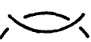
\includegraphics{Figures/Crossings/R2cross.png}}
\newcommand{\RIIItop}{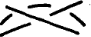
\includegraphics{Figures/Crossings/R3top.png}}
\newcommand{\RIIIbottom}{\raisebox{5pt}{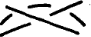
\includegraphics[angle = 180]{Figures/Crossings/R3top.png}}}
\newcommand{\Kcross}{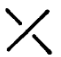
\includegraphics[width = 0.5cm]{Figures/Crossings/crossing.png}}
\newcommand{\Kcrossreflect}{\reflectbox{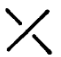
\includegraphics[width = 0.5cm]{Figures/Crossings/crossing.png}}}

\newcommand{\ARes}{\raisebox{-5pt}{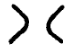
\includegraphics[width = 0.8cm]{Figures/Crossings/A_res.png}}}
\newcommand{\BRes}{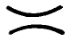
\includegraphics[width = 0.5cm]{Figures/Crossings/B_res.png}}
\newcommand{\plusOne}{\includesvg[width = 0.5cm]{Figures/Crossings/arrow_crossing.svg}}
\newcommand{\minusOne}{\reflectbox{\includesvg[width = 0.5cm]{Figures/Crossings/arrow_crossing.svg}}}


\subsection{4}

Firstly, $P$ is always invariant under ambient isotopy. When the knot diagram is moved around, the crossings do not change and the underlying $4$-valent graphs stay the same. Therefore, the properties of $P$ are the same.  

If $P$ is invariant under Reidermeister II moves and ambient isotopy, $P$ is invariant under Reidermeister III moves. 

This is because of the following:
\begin{align*}
    P(\RIIItop) &= f(A)P(\raisebox{-5pt}{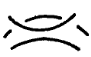
\includegraphics{Figures/Crossings/R3Ares.png}}) + g(A)P(\raisebox{-5pt}{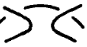
\includegraphics{Figures/Crossings/R3Bres.png}})\\
    &= f(A)P(\raisebox{10pt}{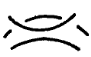
\includegraphics[angle = 180]{Figures/Crossings/R3Ares.png}}) + g(A)P(\raisebox{10pt}{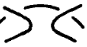
\includegraphics[angle = 180]{Figures/Crossings/R3Bres.png}})\\
    &=P(\RIIIbottom)
\end{align*}
where the third step comes from applying Reidermeister II moves and the ambient isotopy relation.


Now $P$ is invariant under Reidermeister II moves if and only if $fg = 1$ and $h = -f^2 - g^2$. 

\begin{align*}
    P(\RIIcross) &= f(A)P(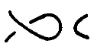
\includegraphics{Figures/Crossings/R2Ares.png}) + g(A) P(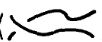
\includegraphics{Figures/Crossings/R2Bres.png})\\
    &= f(A)\left(f(A)P(\ARes) + g(A) P(\raisebox{-5pt}{\includesvg[width = 0.8cm]{Figures/Crossings/R2djcircle.svg}})\right) + g(A)\left(f(A) P(\BRes) + g(A)P(\ARes)\right)\\
    &=f(A)\left(f(A)P(\ARes) + g(A) h(A) P(\ARes)\right) + g(A)\left(f(A) P(\BRes) + g(A)P(\ARes)\right)\\
    &= g fP(\BRes) +(f^2 + fgh + g^2) P(\ARes)
\end{align*}

Since $P$ is a polynomial,$g fP(\BRes) +(f^2 + fgh + g^2) P(\ARes) = P(\BRes)$ if and only if $gf = 1$ and $f^2 + h + g^2 = 0$. Then $h = -f^2 - g^2$.

Therefore, $P$ is invariant under ambient isotopy, Reidermeister II and III moves if and only if $fg = 1$ and $h = -f^2 - g^2$. 

\subsection{5}

We want to show that \[(-A)^{-3w(L \sqcup O)} \langle L \sqcup O \rangle = (-A)^{-3w(L)}(-A^{-2} - A^2)\langle L \rangle\] If this is the case, then setting $t^{1/2} = A^{-2}$ yields $V(L \sqcup O) = (-t^{-1/2} - t^{1/2}) V(L)$.

Firstly, $w(L \sqcup O) = w(L) + w(O)$, as these knots are disjoint. Then $w(O) = 0$ as there are no crossings in $O$. So $w(L \sqcup O) = w(L)$. Next, \[\langle L \sqcup O \rangle = (-A^{-2} - A^2)\langle L \rangle.\] So \[(-A)^{-3w(L \sqcup O)} \langle L \sqcup O \rangle = (-A)^{-3w(L)}(-A^{-2} - A^2)\langle L \rangle.\]

\subsection{6}

We want to show that \[(-A)^{-3w(L^*)}\langle L^* \rangle(A) = (-A)^{3w(L)}\langle L \rangle(A^{-1}).\] If this is the case, then substituting $t^{1/2} = A^{-2}$ yields $V(L^*)(t) = V(L)(t^{-1})$. 

Firstly, $w(L^*) = -w(L)$. This is because for every crossing, \plusOne, which is $+1$ writhe becomes \minusOne, which is $-1$ writhe. 

Next, $\langle L^* \rangle(A) = \langle L \rangle(A^{-1})$. We prove this by induction.
For the base case, if $L$ is the unknot, the $L^*$ is also the unknot so $\langle L^* \rangle(A) = \langle L \rangle(A^{-1}) = 1$. If there is a disjoint unknot, then flipping the link keeps the unknot disjoint. Assume for the induction hypothesis that $\langle L^* \rangle(A) = \langle L \rangle(A^{-1})$, and the knot we are working with is $L \sqcup O$. Then
\[\langle L \sqcup O \rangle(A^{-1}) = (-A^2 - A^{-2}) \langle L \rangle(A^{-1}) = (-A^2 - A^{-2}) \langle L^* \rangle(A) = \langle O \sqcup L^* \rangle(A).\]
This is because $(-A^2 - A^{-2})$ is symmetric when $A \mapsto A^{-1}$.

Finally,  \[\langle \Kcross \rangle(A^{-1}) = A^{-1} \langle \ARes \rangle(A^{-1}) + A \langle \BRes \rangle(A^{-1}).\] By induction, \[\langle \ARes \rangle(A^{-1}) = \langle \ARes^* \rangle(A)\]
and  \[\langle \BRes \rangle(A^{-1}) = \langle \BRes^* \rangle(A).\]
But if $L$ has \Kcross, then \Kcross becomes \Kcrossreflect in $L^*$. So in $L^*$, \ARes and \BRes are swapped, so \[\langle \Kcrossreflect \rangle(A) = A \langle \BRes^* \rangle(A) + A^{-1} \langle \ARes^* \rangle(A) = A \langle \BRes \rangle(A^{-1}) + A^{-1} \langle \ARes \rangle(A^{-1}) = \langle \Kcross \rangle(A^{-1}).\] Therefore, $\langle L^* \rangle(A) = \langle L \rangle(A^{-1})$. Finally, $(-A)^{-3w(L^*)}\langle L^* \rangle(A) = (-A)^{3w(L)}\langle L \rangle(A^{-1})$, so $V(L^*)(t) = V(L)(t^{-1})$. 

\subsection{7}
Exercise 6 implies that if a knot $K$ is amphichiral, then $V(K)(t) = V(K)(t^{-1})$. 

The right trefoil has Jones polynomial $-t^4 + t^3 + t$, from Lickorish (p 29). By exercise 6,  $t \mapsto t^{-1}$ is the Jones polynomial of the left trefoil, which is $-t^{-4} + t^{-3} + t^{-1}$. Therefore, the left trefoil is not amphichiral.

\subsection{8}

First, we want to show that $w(K_1 \# K_2) = w(K_1) + w(K_2)$ and $\langle K_1 \# K_2 \rangle = \langle K_1 \rangle\langle K_2 \rangle$. If this holds, then \[(-A)^{-3w(K_1 \# K_2)} \langle K_1 \# K_2 \rangle = (-A)^{-3w(K_1)} \langle K_1 \rangle (-A)^{-3w(K_2)} \langle K_2 \rangle,\] which implies that $V(K_1 \# K_2) = V(K_1) V(K_2)$ by setting $t^{1/2} = A^{-2}$. 

Firstly, $w(K_1 \# K_2) = w(K_1) + w(K_2)$ since every crossing in $w(K_1 \# K_2)$ is either in $K_1$ or $K_2$, so the writhe number is additive. 

We have from the sum of states formula that:
\[\langle K_1 \# K_2\rangle = \sum_{s}\left[A^{d(s)}(-A^2 - A^{-2})^{|s| - 1} \right],\] where $d(s)$ is the sum of $A - B$ turns for each crossing and $|s|$ are the number of disjoint circles at the end. 

We can decompose every state $s$ into two substates $s_1, s_2$ where $s_1$ are on crossings in $K_1$ and $s_2$ are on crossings in $K_2$. Each $s_1$ is paired with an $s_2$ to form all $s$, and in fact every combination of $s_1$ and $s_2$ appears exactly once. Secondly, since $d(s)$ counts the number of $A - B$ crossings, $d(s) = d(s_1) + d(s_2)$. Finally, the number of disjoint circles of $s_1$ and $s_2$ is equal to $s$ except that two circles, one from $K_1$ and one from $K_2$ are linked together from the connected sum operation. Then $|s| = |s_1| + |s_2| - 1$. So

\begin{align*}
    \langle K_1 \# K_2\rangle &= \sum_{s}\left[A^{d(s)}(-A^2 - A^{-2})^{|s| - 1} \right]\\
    &= \sum_{s_1 + s_2}\left[A^{d(s_1) + d(s_2)}(-A^2 - A^{-2})^{|s_1|- 1 + |s_2| - 1} \right]\\
    &= \sum_{s_1 + s_2}\left[A^{d(s_1)}(-A^2 - A^{-2})^{|s_1|- 1} \right] \left[A^{d(s_2)}(-A^2 - A^{-2})^{|s_2|- 1} \right]\\
    &= \sum_{s_1}\left[A^{d(s_1)}(-A^2 - A^{-2})^{|s_1|- 1} \right] \sum_{s_2}\left[A^{d(s_2)}(-A^2 - A^{-2})^{|s_2|- 1} \right]\\
    &= \langle K_1 \rangle \langle K_2 \rangle
\end{align*}
Therefore,  $V(K_1 \# K_2) = V(K_1) V(K_2)$.
\end{document}
